\documentclass{article} % The document class
\usepackage{graphicx} % Required for inserting images
\usepackage{geometry} % Required for modifying paper layout
\usepackage{amsmath} % Required for inserting math formulae
\usepackage{listings} % Required for inserting codes
\usepackage{xcolor} % Required for adding colors
\usepackage{hyperref} % Required for inserting hyperlinks
\usepackage{indentfirst} % Required for indent the first paragraph
\usepackage{booktabs} % Required for inserting booktabs table
\usepackage{float} % Required for editing float figures

\geometry{a4paper,scale = 0.8} % Modifying the paper layout
\hypersetup{ % hyperlinks setup
    hidelinks,
    colorlinks = true,
    allcolors = blue,
    pdfstartview = Fit,
    breaklinks = true
}
\lstset{ % code style setup
	basicstyle          =   \sffamily,          
	keywordstyle        =   \bfseries,          
	commentstyle        =   \rmfamily\itshape,  
	stringstyle         =   \ttfamily,  
	flexiblecolumns,                
	showspaces          =   false,  
	numberstyle         =   \zihao{-5}\ttfamily,    
	showstringspaces    =   false,
	captionpos          =   t,      
}

\title{\ttfamily{Example}}
\author{\sffamily{jan\_chen}}
\date{\texttt{September 2023}}

\setlength{\parindent}{2em}
\setlength{\parskip}{0.5em}
\linespread{1.5}

\begin{document}

\maketitle

\tableofcontents

\section{Section}
\subsection{Subsection}
\subsubsection{Subsubsection}

{\large \textbf{This}} is the \textit{Pythagorean theorem}:
\begin{equation}
    a^2 + b^2 = c^2
\end{equation}
where $a$, $b$ are \textit{right-angle sides} and $c$ is \textit{hypotenuse}.

This image illustrates the theorem:
\begin{figure}[H]
    \centering
    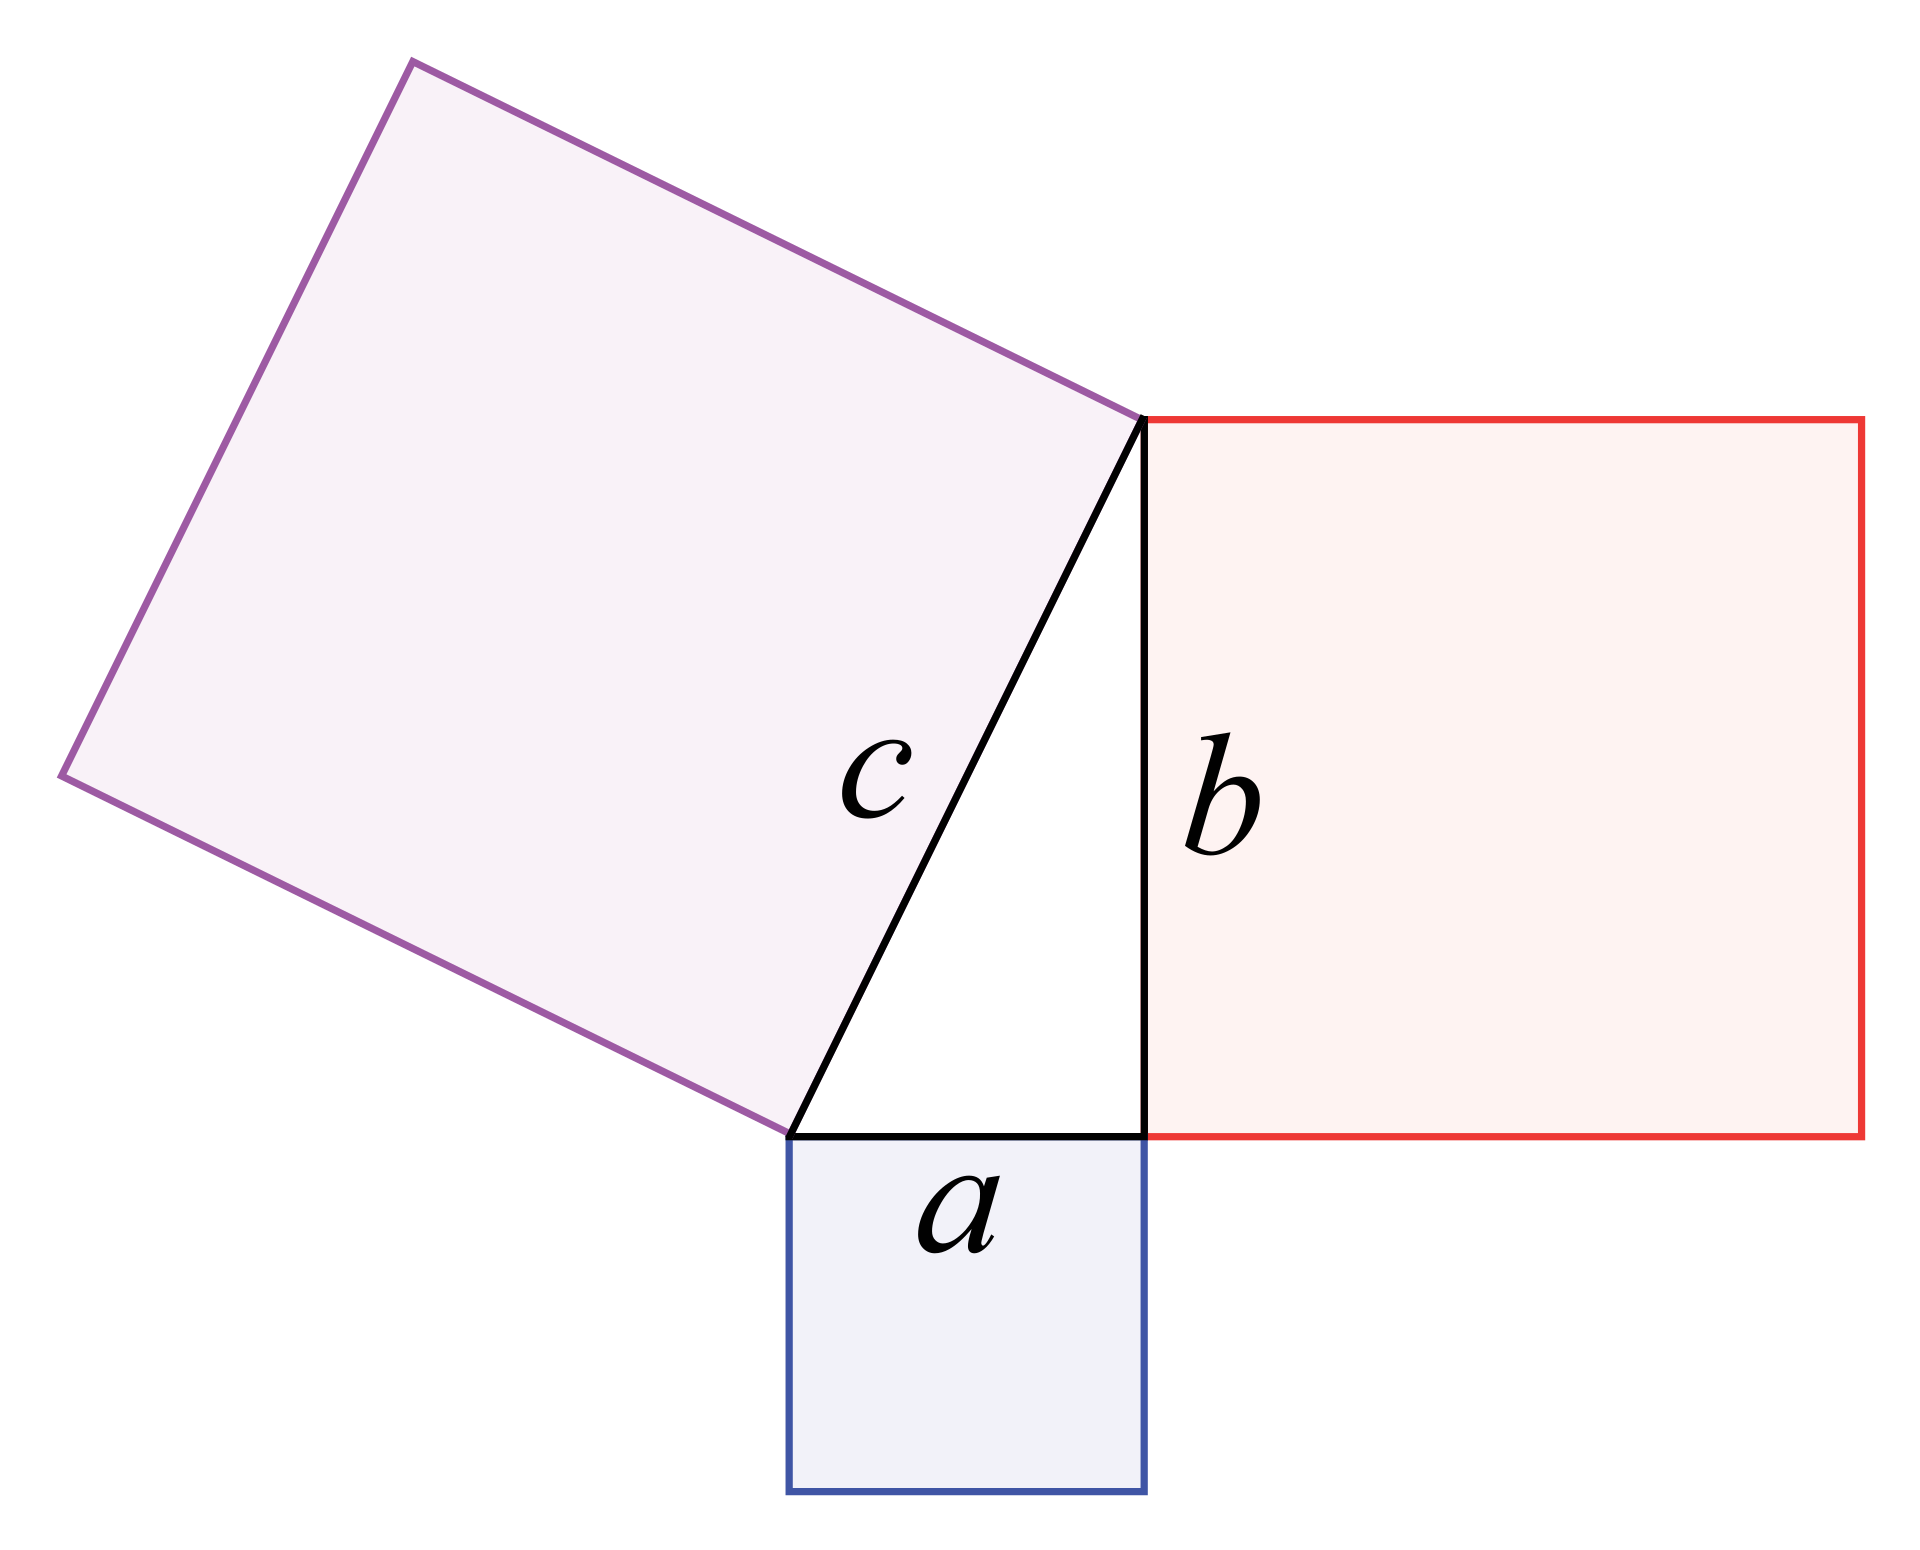
\includegraphics[scale = 0.06]{image/pythagorean th.png}
    \caption{Pythagorean Theorem}
    \label{pt}
\end{figure}

In Figure (\ref{pt}), the sum of the area of the red and blue rectangles equals that of the purple rectangle. Eli Maor has introduced the history of the theorem and its significance in his book \cite{ref1}: \href{https://books.google.com.sg/books?id=XuWZDwAAQBAJ&dq=pythagorean+theorem&lr=&hl=zh-CN&source=gbs_navlinks_s}{The Pythagorean Theorem: A 4000-Year History} and Kadison described the finite case in his article \cite{ref2} \href{https://doi.org/10.1073/pnas.032677199}{The Pythagorean Theorem: I. The finite case}.
This table gives some common pythagorean numbers:

\begin{table}[H]
\centering
\setlength{\tabcolsep}{10mm}
\begin{tabular}{@{}ccc@{}}
\toprule
a & b  & c  \\ \midrule
3 & 4  & 5  \\
5 & 12 & 13 \\
7 & 24 & 25 \\ \bottomrule
\end{tabular}
\caption{Pythagorean numbers}
\label{tab:my-table}
\end{table}

James Abram Garfield\footnote{Garfield became US president five years after he gave this proof} gave his proof of the theorem like this:

In Right trapezoid ABDE:
\begin{figure}[H]
    \centering
    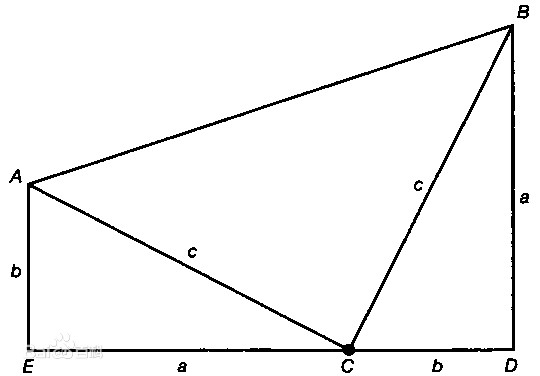
\includegraphics[scale = 0.3]{image/proof.jpg}
    \caption{President's proof}
    \label{pf}
\end{figure}
\begin{align*}
    \angle{AEC} = \angle{CDB} = 90^{\circ}\quad \Delta{AEC}\cong \Delta{CDB}\quad AE = CD = b\quad CE = BD = a\quad AC = BC = c
\end{align*}
\begin{align*}
    S_{\Delta AEC} &= S_{\Delta CDB} =\frac{ab}{2}\\
    S_{\Delta ACB} &= \frac{c^2}{2}\\
    S_{AEDB} &= \frac{(a+b)\times(a+b)}{2}\\
\end{align*}

Since
\begin{align*}
    S_{\Delta AEC} + S_{\Delta CDB}+S_{\Delta ACB} &= S_{AEDB}\\
    \Longrightarrow \frac{ab}{2}+\frac{ab}{2}+\frac{c^2}{2}&=\frac{(a+b)^2}{2}\\
    ab +\frac{ac}{2} &= ab + \frac{a^2+b^2}{2}
\end{align*}

Therefore
\begin{align*}
    c^2 = a^2 + b^2
\end{align*}

We can also use Pythagorean Th. to tell the shape of a triangle i.e.
\begin{equation*}
    \text{Given any triangle }\Delta ABC 
    \begin{cases}
    \text{ right triangle }& \text{if } c^2 = a^2 + b^2\\
    \text{ acute triangle }& \text{if } c^2 < a^2 + b^2\\
    \text{ obtuse triangle }& \text{if } c^2 > a^2 + b^2
    \end{cases}
\end{equation*}

To know more about Pythagorean Th., please refer to \href{https://www.wikiwand.com/en/Pythagorean_theorem}{wikipedia}


\clearpage
\bibliographystyle{plain}
\bibliography{ref}



\end{document}
